\documentclass[11pt]{article}
\usepackage[textwidth=18.0cm, textheight=23.0cm, top=2.0cm]{geometry}
\usepackage{pst-all}
\usepackage{amssymb}
\usepackage{tikz}
\usepackage{underscore}\begin{document}
\pagestyle{empty}


ClassName: \underline{\textbf{Class_10.2bp-0}}
\par
BinSize: \underline{\textbf{100 × 100}}
\par
ReduceSize: \underline{\textbf{100 × 100}}
\par
TypeNum: \underline{\textbf{19}}
\par
Num: \underline{\textbf{20}}
\par
OutS: \underline{\textbf{60000}}
\par
InS: \underline{\textbf{50083}}
\par
Rate: \underline{\textbf{0.835}}
\par
UB: \underline{\textbf{6}}
\par
LB0: \underline{\textbf{6}}
\par
LB: \underline{\textbf{6}}
\par
LBWithCut: \underline{\textbf{6}}
\par
NodeCut: \underline{\textbf{0}}
\par
ExtendedNodeCnt: \underline{\textbf{1}}
\par
GenNodeCnt: \underline{\textbf{1}}
\par
PrimalNode: \underline{\textbf{0}}
\par
ColumnCount: \underline{\textbf{6}}
\par
TotalCutCount: \underline{\textbf{0}}
\par
RootCutCount: \underline{\textbf{0}}
\par
LPSolverCnt: \underline{\textbf{1}}
\par
PricingSolverCnt: \underline{\textbf{0}}
\par
BranchAndBoundNum: \underline{\textbf{1}}
\par
isOpt: \underline{\textbf{true}}
\par
TimeOnInitSolution: \underline{\textbf{0.010 s}}
\par
TimeOnPrimal: \underline{\textbf{0.000 s}}
\par
TimeOnPricing: \underline{\textbf{0.000 s}}
\par
TimeOnRmp: \underline{\textbf{0.078 s}}
\par
TotalTime: \underline{\textbf{0.135 s}}
\par
\newpage


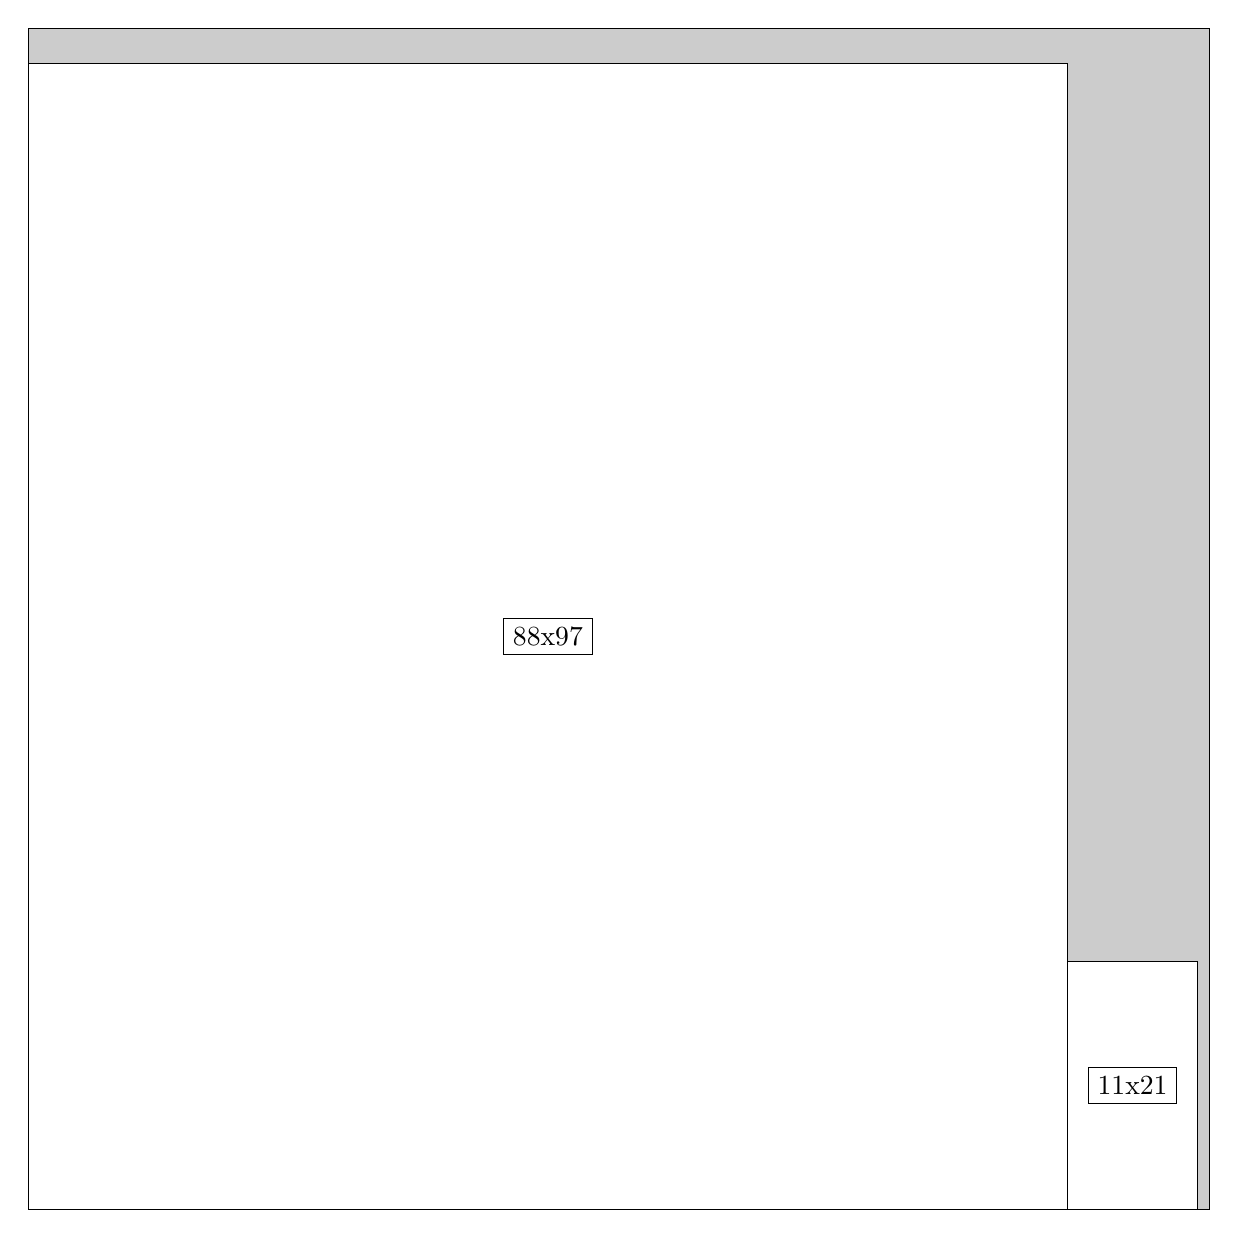
\begin{tikzpicture}[shorten >=1pt,scale=1.0,every node/.style={scale=1.0},->]
\tikzstyle{vertex}=[circle,fill=black!25,minimum size=14pt,inner sep=0pt]
\filldraw[fill=gray!40!white, draw=black] (0,0) rectangle (15.0,15.0);
\foreach \name/\x/\y/\w/\h in {88x97/0.0/0.0/13.2/14.549999999999999,11x21/13.2/0.0/1.65/3.15}
\filldraw[fill=white!40!white, draw=black] (\x,\y) rectangle node[draw] (\name) {\name} ++(\w,\h);
\end{tikzpicture}


w =88 , h =97 , x =0 , y =0 , v =8536
\par
w =11 , h =21 , x =88 , y =0 , v =231
\par
\newpage


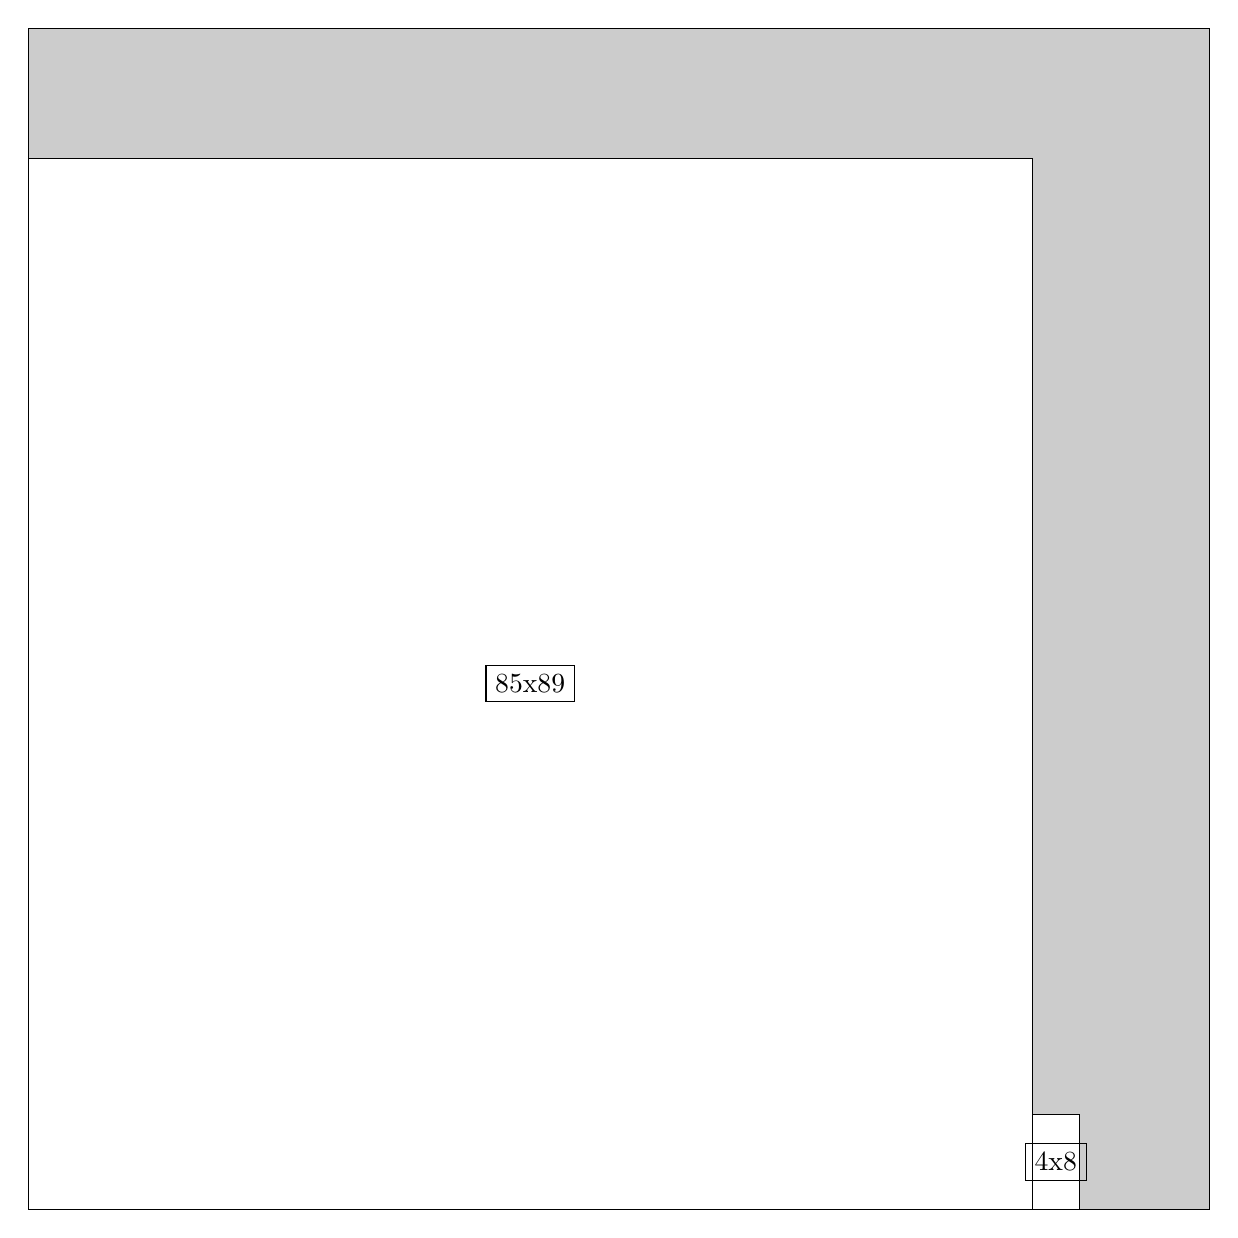
\begin{tikzpicture}[shorten >=1pt,scale=1.0,every node/.style={scale=1.0},->]
\tikzstyle{vertex}=[circle,fill=black!25,minimum size=14pt,inner sep=0pt]
\filldraw[fill=gray!40!white, draw=black] (0,0) rectangle (15.0,15.0);
\foreach \name/\x/\y/\w/\h in {85x89/0.0/0.0/12.75/13.35,4x8/12.75/0.0/0.6/1.2}
\filldraw[fill=white!40!white, draw=black] (\x,\y) rectangle node[draw] (\name) {\name} ++(\w,\h);
\end{tikzpicture}


w =85 , h =89 , x =0 , y =0 , v =7565
\par
w =4 , h =8 , x =85 , y =0 , v =32
\par
\newpage


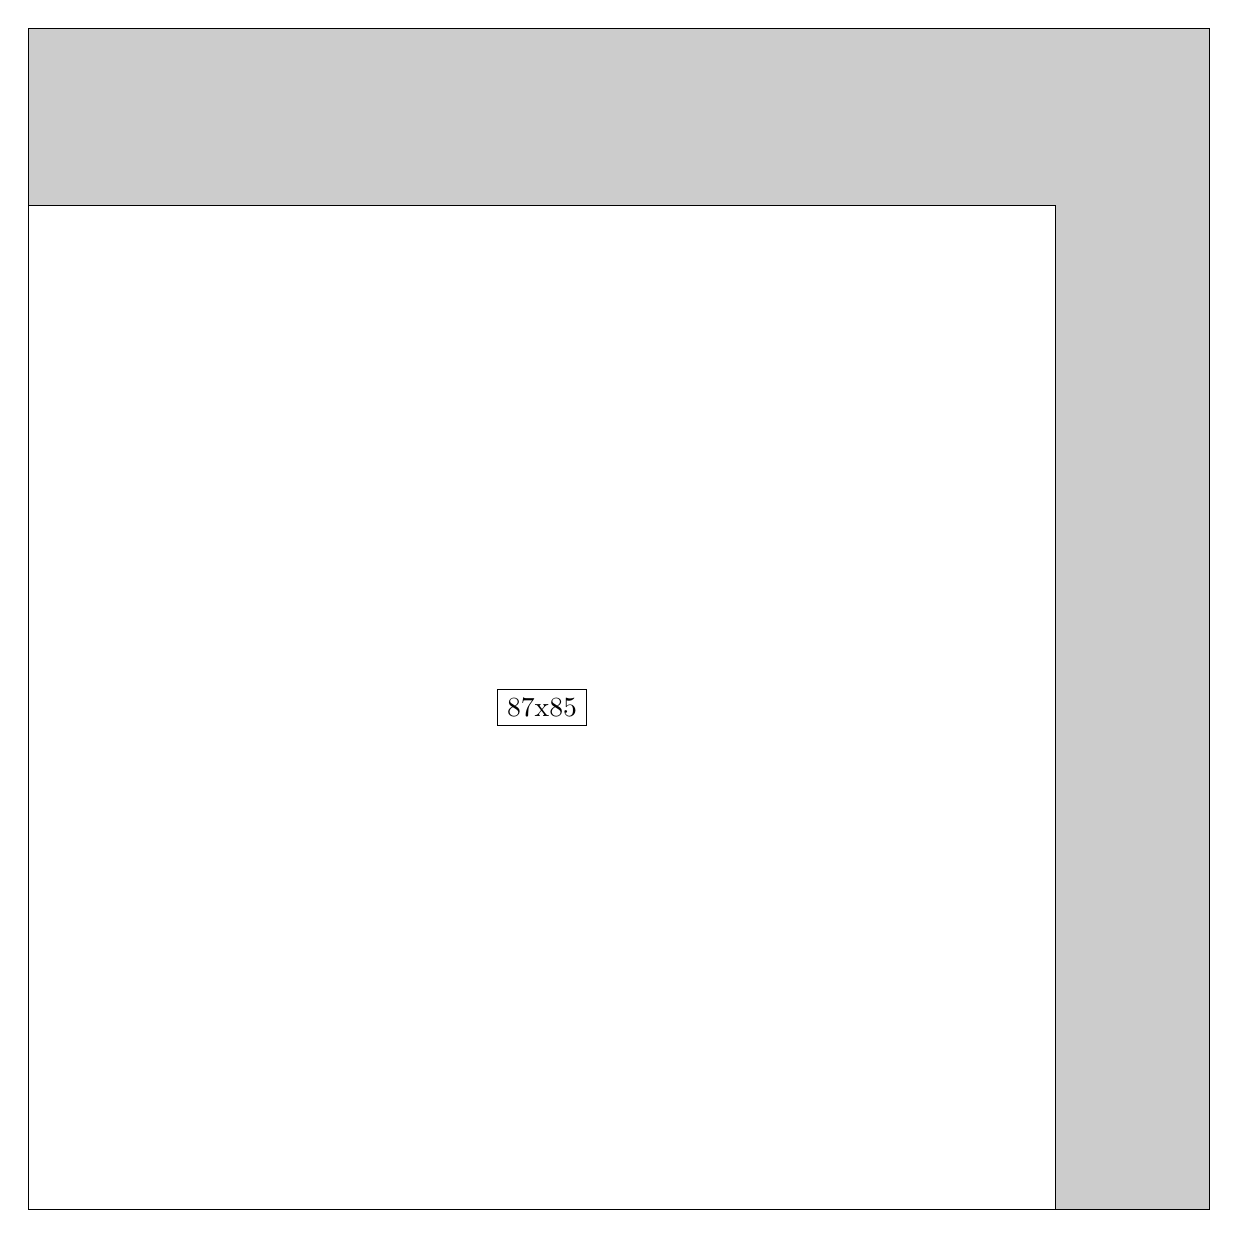
\begin{tikzpicture}[shorten >=1pt,scale=1.0,every node/.style={scale=1.0},->]
\tikzstyle{vertex}=[circle,fill=black!25,minimum size=14pt,inner sep=0pt]
\filldraw[fill=gray!40!white, draw=black] (0,0) rectangle (15.0,15.0);
\foreach \name/\x/\y/\w/\h in {87x85/0.0/0.0/13.049999999999999/12.75}
\filldraw[fill=white!40!white, draw=black] (\x,\y) rectangle node[draw] (\name) {\name} ++(\w,\h);
\end{tikzpicture}


w =87 , h =85 , x =0 , y =0 , v =7395
\par
\newpage


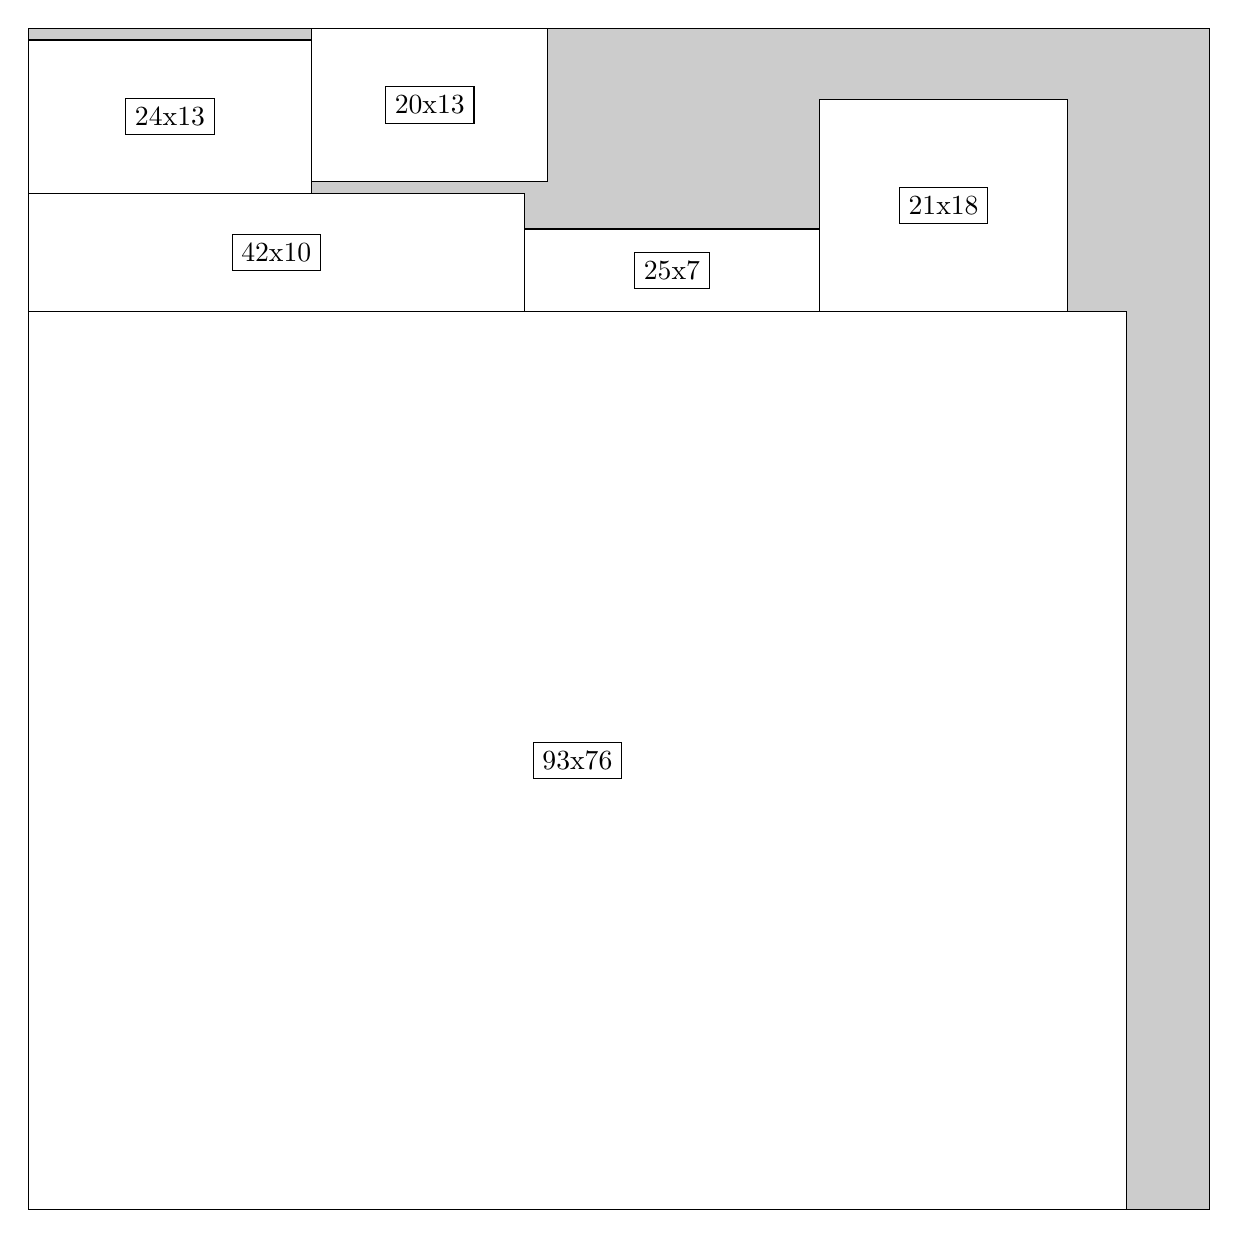
\begin{tikzpicture}[shorten >=1pt,scale=1.0,every node/.style={scale=1.0},->]
\tikzstyle{vertex}=[circle,fill=black!25,minimum size=14pt,inner sep=0pt]
\filldraw[fill=gray!40!white, draw=black] (0,0) rectangle (15.0,15.0);
\foreach \name/\x/\y/\w/\h in {93x76/0.0/0.0/13.95/11.4,42x10/0.0/11.4/6.3/1.5,24x13/0.0/12.9/3.5999999999999996/1.95,21x18/10.049999999999999/11.4/3.15/2.6999999999999997,20x13/3.5999999999999996/13.049999999999999/3.0/1.95,25x7/6.3/11.4/3.75/1.05}
\filldraw[fill=white!40!white, draw=black] (\x,\y) rectangle node[draw] (\name) {\name} ++(\w,\h);
\end{tikzpicture}


w =93 , h =76 , x =0 , y =0 , v =7068
\par
w =42 , h =10 , x =0 , y =76 , v =420
\par
w =24 , h =13 , x =0 , y =86 , v =312
\par
w =21 , h =18 , x =67 , y =76 , v =378
\par
w =20 , h =13 , x =24 , y =87 , v =260
\par
w =25 , h =7 , x =42 , y =76 , v =175
\par
\newpage


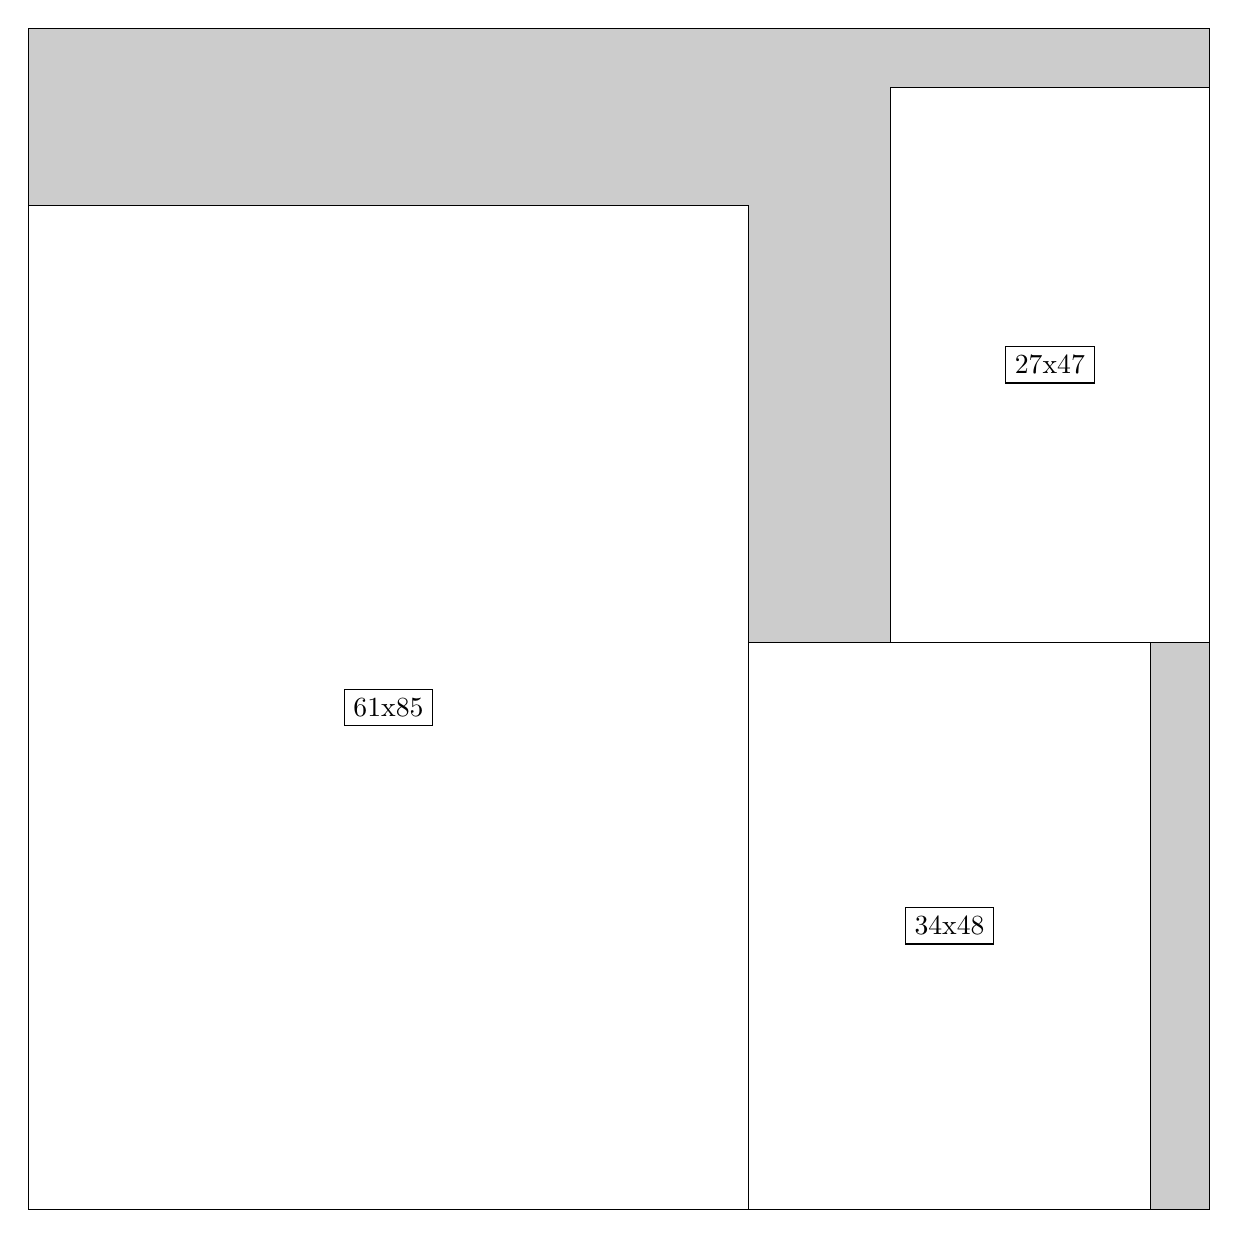
\begin{tikzpicture}[shorten >=1pt,scale=1.0,every node/.style={scale=1.0},->]
\tikzstyle{vertex}=[circle,fill=black!25,minimum size=14pt,inner sep=0pt]
\filldraw[fill=gray!40!white, draw=black] (0,0) rectangle (15.0,15.0);
\foreach \name/\x/\y/\w/\h in {61x85/0.0/0.0/9.15/12.75,34x48/9.15/0.0/5.1/7.199999999999999,27x47/10.95/7.199999999999999/4.05/7.05}
\filldraw[fill=white!40!white, draw=black] (\x,\y) rectangle node[draw] (\name) {\name} ++(\w,\h);
\end{tikzpicture}


w =61 , h =85 , x =0 , y =0 , v =5185
\par
w =34 , h =48 , x =61 , y =0 , v =1632
\par
w =27 , h =47 , x =73 , y =48 , v =1269
\par
\newpage


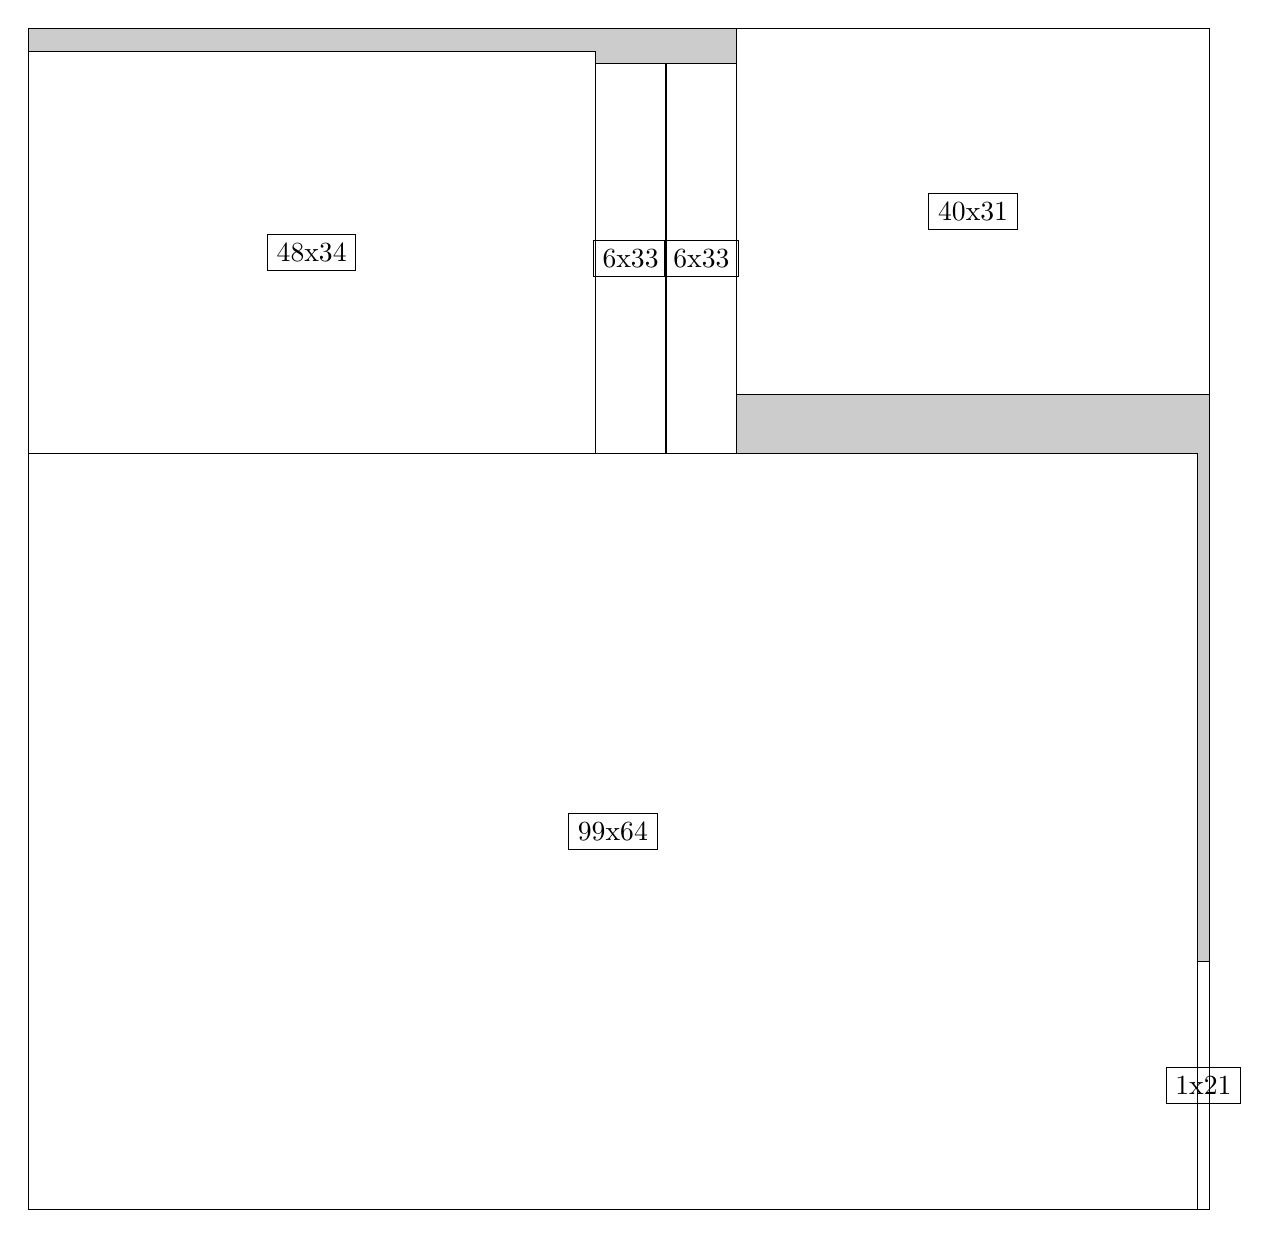
\begin{tikzpicture}[shorten >=1pt,scale=1.0,every node/.style={scale=1.0},->]
\tikzstyle{vertex}=[circle,fill=black!25,minimum size=14pt,inner sep=0pt]
\filldraw[fill=gray!40!white, draw=black] (0,0) rectangle (15.0,15.0);
\foreach \name/\x/\y/\w/\h in {99x64/0.0/0.0/14.85/9.6,48x34/0.0/9.6/7.199999999999999/5.1,40x31/9.0/10.35/6.0/4.6499999999999995,6x33/7.199999999999999/9.6/0.8999999999999999/4.95,6x33/8.1/9.6/0.8999999999999999/4.95,1x21/14.85/0.0/0.15/3.15}
\filldraw[fill=white!40!white, draw=black] (\x,\y) rectangle node[draw] (\name) {\name} ++(\w,\h);
\end{tikzpicture}


w =99 , h =64 , x =0 , y =0 , v =6336
\par
w =48 , h =34 , x =0 , y =64 , v =1632
\par
w =40 , h =31 , x =60 , y =69 , v =1240
\par
w =6 , h =33 , x =48 , y =64 , v =198
\par
w =6 , h =33 , x =54 , y =64 , v =198
\par
w =1 , h =21 , x =99 , y =0 , v =21
\par
\newpage


\end{document}